\appendix

\section{Datasets}
\label{app:datasets}
Due to space limitations in the main manuscript, we provide here a detailed description of the industrial anomaly detection datasets used in our experiments: MVTec-AD~\cite{Bergmann_2019_CVPR}, VisA~\cite{VisA}, MPDD~\cite{mpdd}, and Real-IAD~\cite{wang2024realiadrealworldmultiviewdataset}. Key dataset statistics, including the number of defect types, object categories, and the proportion of single- and multi-defect images, are summarized in \cref{tab:dataset_summary}. For all datasets, each defect instance is mapped to a unified defect taxonomy as defined in \crefrange{tab:mvtec-mapping1}{tab:real-iad-mapping2}.
MVTec-AD includes common industrial items such as bottles, cables, zippers, and hazelnuts. VisA contains a mixture of everyday products such as chewing gum and macaroni, as well as more complex components like printed circuit boards. MPDD focuses primarily on industrial parts, including metal brackets, tubes, and machined components. Real-IAD contains a broad range of real-world consumer and industrial items such as audio jacks, switches, bottle caps, and plastic toys.

% Overview of Datasets
\begin{table*}
\centering
\setlength{\tabcolsep}{5pt}
\caption[Overview of the datasets used for evaluation.]{Overview of the datasets used for evaluation. The third column lists distinct defects, while the fourth column counts compound defects treated as separate categories.}
\label{tab:dataset_summary}
\begin{tabular}{cccccc}
\toprule
\textbf{Dataset} & \textbf{Objects} & \textbf{\begin{tabular}[c]{@{}c@{}}Unique \\ Defect Types\end{tabular}} & \textbf{\begin{tabular}[c]{@{}c@{}}Defect Types \\ Incl. Combinations\end{tabular}} & \textbf{\begin{tabular}[c]{@{}c@{}}Single Defect \\ Images\end{tabular}} & \textbf{\begin{tabular}[c]{@{}c@{}}Multi Defect \\ Images\end{tabular}} \\
\midrule
MVTec-AD  & 15 & 16 & 38   & 1,200  & 58   \\
VisA      & 12 & 14 & 56   & 923    & 277  \\
MPDD      & 6  & 6  & 7    & 265    & 17   \\
Real-IAD  & 30 & 9  & 9    & 51,329 & 0    \\
\bottomrule
\end{tabular}
\end{table*}

% MVTec Mapping
\begin{table}
\centering
\footnotesize
\caption{Defect taxonomy for the MVTec-AD dataset (Part I).}
\label{tab:mvtec-mapping1}
\begin{tabular}{@{}ccc@{}}
\toprule
\textbf{Product} & \textbf{Original Defect Types} & \textbf{Mapped Defect Types} \\
\midrule

\multirow{3}{*}{Bottle}
 & Broken Large & Broken \\
 & Broken Small & Broken \\
 & Contamination & Contamination \\

\midrule
\multirow{8}{*}{Cable}
 & Bent Wire & Bent \\
 & Cable Swap & Misplaced \\
 & Combined & Combination of Defects \\
 & Cut Inner Insulation & Cut \\
 & Cut Outer Insulation & Cut \\
 & Missing Cable & Missing \\
 & Missing Wire & Missing \\
 & Poke Insulation & Poke \\

\midrule
\multirow{5}{*}{Capsule}
 & Crack & Crack \\
 & Faulty Imprint & Scratch \\
 & Poke & Crack \\
 & Scratch & Scratch \\
 & Squeeze & Deformed \\

\midrule
\multirow{5}{*}{Carpet}
 & Color & Color \\
 & Cut & Tear \\
 & Hole & Hole \\
 & Metal Contamination & Contamination \\
 & Thread & Contamination \\

\midrule
\multirow{4}{*}{Hazelnut}
 & Crack & Crack \\
 & Cut & Cut \\
 & Hole & Hole \\
 & Print & Color \\

\midrule
\multirow{5}{*}{Grid}
 & Bent & Bent \\
 & Broken & Broken \\
 & Glue & Contamination \\
 & Metal Contamination & Contamination \\
 & Thread & Contamination \\

\midrule
\multirow{5}{*}{Leather}
 & Color & Color \\
 & Cut & Cut \\
 & Fold & Fold \\
 & Glue & Contamination \\
 & Poke & Poke \\

\midrule
\multirow{4}{*}{Metal Nut}
 & Bent & Bent \\
 & Color & Color \\
 & Flip & Misplaced \\
 & Scratch & Scratch \\

\midrule
\multirow{7}{*}{Pill}
 & Color & Color \\
 & Combined & Combination of Defects \\
 & Contamination & Contamination \\
 & Crack & Crack \\
 & Faulty Imprint & Scratch \\
 & Pill Type & Color \\
 & Scratch & Scratch \\

\midrule
\multirow{5}{*}{Screw}
 & Manipulated Front & Bent Head / Broken Tip \\
 & Scratch Head & Damaged \\
 & Scratch Neck & Damaged \\
 & Thread Side & Damaged \\
 & Thread Top & Damaged \\

\bottomrule
\end{tabular}
\end{table}

\begin{table}
\centering
\footnotesize
\caption{Defect taxonomy for the MVTec-AD dataset (Part II).}
\label{tab:mvtec-mapping2}
\begin{tabular}{@{}ccc@{}}
\toprule
\textbf{Product} & \textbf{Original Defect Types} & \textbf{Mapped Defect Types} \\
\midrule

\multirow{5}{*}{Tile}
 & Crack & Crack \\
 & Glue Strip & Contamination \\
 & Gray Stroke & Color \\
 & Oil & Contamination \\
 & Rough & Scratch \\

\midrule
\multirow{1}{*}{Toothbrush}
 & Defective & Bent / Contamination / Missing \\

\midrule
\multirow{4}{*}{Transistor}
 & Bent Lead & Bent \\
 & Cut Lead & Broken \\
 & Damaged Case & Damaged \\
 & Misplaced & Misplaced \\

\midrule
\multirow{5}{*}{Wood}
 & Color & Color \\
 & Combined & Combination of Defects \\
 & Hole & Hole \\
 & Liquid & Contamination \\
 & Scratch & Scratch \\

\midrule
\multirow{7}{*}{Zipper}
 & Broken Teeth & Broken \\
 & Combined & Combination of Defects \\
 & Fabric Border & Tear \\
 & Fabric Interior & Tear \\
 & Rough & Contamination \\
 & Split Teeth & Deformed \\
 & Squeezed Teeth & Deformed \\

\bottomrule
\end{tabular}
\end{table}

% VisA Mapping
\begin{table}
\centering
\scriptsize
\renewcommand{\arraystretch}{0.9}
\caption{Defect taxonomy for the VisA dataset (Part I).}
\label{tab:visa-mapping1}
\begin{tabular}{@{}ccc@{}}
\toprule
\textbf{Product} & \textbf{Original Defect Types} & \textbf{Mapped Defect Types} \\
\midrule

\multirow{8}{*}{Candle}
 & Chunk of Wax Missing & Hole \\
 & Damaged Corner of Packaging & Damaged \\
 & Different Colour Spot & Color \\
 & Extra Wax in the Candle & Contamination \\
 & Foreign Particals on the Candle & Color \\
 & Wax Melded out of the Candle & Melded \\
 & Weird Candle Wick & Weird Wick \\
 & Combined & Combination of Defects \\

\midrule
\multirow{6}{*}{Capsules}
 & Bubble & Bubble \\
 & Discolor & Color \\
 & Scratch & Scratch \\
 & Leak & Contamination \\
 & Misshape & Deformed \\
 & Combined & Combination of Defects \\

\midrule
\multirow{9}{*}{Cashew}
 & Burnt & Color \\
 & Corner or Edge Breakage & Broken \\
 & Different Colour Spot & Color \\
 & Middle Breakage & Broken \\
 & Same Colour Spot & Color \\
 & Small Holes & Hole \\
 & Small Scratches & Scratch \\
 & Stuck Together & Misplaced \\
 & Combined & Combination of Defects \\

\midrule
\multirow{6}{*}{Chewinggum}
 & Chunk of Gum Missing & Broken \\
 & Corner Missing & Broken \\
 & Scratches & Scratch \\
 & Similar Colour Spot & Color \\
 & Small Cracks & Crack \\
 & Combined & Combination of Defects \\

\midrule
\multirow{8}{*}{Fryum}
 & Burnt & Color \\
 & Corner or Edge Breakage & Broken \\
 & Different Colour Spot & Color \\
 & Fryum Stuck Together & Misplaced \\
 & Middle Breakage & Broken \\
 & Similar Colour Spot & Color \\
 & Small Scratches & Scratch \\
 & Combined & Combination of Defects \\

\bottomrule
\end{tabular}
\end{table}

\begin{table}
\centering
\scriptsize
\renewcommand{\arraystretch}{0.9}
\caption{Defect taxonomy for the VisA dataset (Part II).}
\label{tab:visa-mapping2}
\begin{tabular}{@{}ccc@{}}
\toprule
\textbf{Product} & \textbf{Original Defect Types} & \textbf{Mapped Defect Types} \\
\midrule

\multirow{7}{*}{Macaroni1}
 & Chip Around Edge and Corner & Broken \\
 & Different Colour Spot & Color \\
 & Similar Colour Spot & Color \\
 & Small Cracks & Crack \\
 & Middle Breakage & Hole \\
 & Small Scratches & Scratch \\
 & Combined & Combination of Defects \\

\midrule

\multirow{7}{*}{Macaroni2}
 & Breakage down the Middle & Hole \\
 & Color Spot Similar to the Object & Color \\
 & Different Color Spot & Color \\
 & Small Chip Around Edge & Broken \\
 & Small Cracks & Crack \\
 & Small Scratches & Scratches \\
 & Combined & Combination of Defects \\

\midrule
\multirow{5}{*}{pcb1}
 & Bent & Bent \\
 & Melt & Contamination \\
 & Missing & Missing \\
 & Scratch & Scratch \\
 & Combined & Combination of Defects \\

\midrule
\multirow{5}{*}{pcb2}
 & Bent & Bent \\
 & Melt & Contamination \\
 & Missing & Missing \\
 & Scratch & Scratch \\
 & Combined & Combination of Defects \\

\midrule
\multirow{5}{*}{pcb3}
 & Bent & Bent \\
 & Melt & Contamination \\
 & Missing & Missing \\
 & Scratch & Scratch \\
 & Combined & Combination of Defects \\

\midrule
\multirow{8}{*}{pcb4}
 & Burnt & Contamination \\
 & Scratch & Scratch \\
 & Damage & Damaged \\
 & Dirt & Contamination \\
 & Extra & Contamination \\
 & Missing & Missing \\
 & Wrong Place & Contamination \\
 & Combined & Combination of Defects \\

\midrule
\multirow{8}{*}{Pipe Fryum}
 & Burnt & Color \\
 & Corner and Edge Breakage & Broken \\
 & Different Colour Spot & Color \\
 & Similar Colour Spot & Color \\
 & Small Scratches & Scratch \\
 & Stuck Together & Misplaced \\
 & Small Cracks & Crack \\
 & Combined & Combination of Defects \\

\bottomrule
\end{tabular}
\end{table}

% MPDD Mapping
\begin{table}
\centering
\caption{Defect taxonomy for the MPDD dataset.}
\footnotesize
\label{tab:mpdd-mapping}
\begin{tabular}{@{}ccc@{}}
\toprule
\textbf{Product} & \textbf{Original Defects Types}                                                 & \textbf{Mapped Defect Types}                                           \\ \midrule
Bracket Black    & \begin{tabular}[c]{@{}c@{}}Hole\\ Scratch\end{tabular}                           & \begin{tabular}[c]{@{}c@{}}Hole\\ Scratch\end{tabular}                 \\ \midrule
Bracket Brown    & \begin{tabular}[c]{@{}c@{}}Bend and Parts Mismatch\\ Parts Mismatch\end{tabular} & \begin{tabular}[c]{@{}c@{}}Bent and Misplaced\\ Misplaced\end{tabular} \\ \midrule
Bracket White    & \begin{tabular}[c]{@{}c@{}}Defective Painting\\ Scratches\end{tabular}           & \begin{tabular}[c]{@{}c@{}}Contamination\\ Scratch\end{tabular}        \\ \midrule
Connector        & Parts Mismatch                                                                   & Missing                                                                \\ \midrule
Metal Plate      & \begin{tabular}[c]{@{}c@{}}Major Rust\\ Total Rust\\ Scratch\end{tabular}        & \begin{tabular}[c]{@{}c@{}}Color\\ Color\\ Scratch\end{tabular}        \\ \midrule
Tubes            & Anomalous                                                                        & Deformed                                                               \\ \bottomrule
\end{tabular}
\end{table}

% Real-IAD Mapping
\begin{table}
\centering
\footnotesize
\renewcommand{\arraystretch}{0.7}
\caption{Defect taxonomy for the Real-IAD dataset (Part I).}
\label{tab:real-iad-mapping1}
\begin{tabular}{@{}ccc@{}}
\toprule
\textbf{Product} & \textbf{Original Defect Types} & \textbf{Mapped Defect Types} \\
\midrule

\multirow{4}{*}{Audiojack}
 & Contamination & Color \\
 & Missing Parts & Broken \\
 & Deformation & Bent \\
 & Scratch & Scratch \\

\midrule
\multirow{4}{*}{Bottle Cap}
 & Contamination & Color \\
 & Missing Parts & Broken \\
 & Scratch & Scratch \\
 & Pit & Hole \\

\midrule
\multirow{4}{*}{Button Battery}
 & Scratch & Scratch \\
 & Abrasion & Abrasion \\
 & Contamination & Color \\
 & Pit & Color \\

\midrule
\multirow{4}{*}{End Cap}
 & Damage & Broken \\
 & Missing Parts & Broken \\
 & Contamination & Color \\
 & Scratch & Scratch \\

\midrule
\multirow{4}{*}{Eraser}
 & Contamination & Color \\
 & Scratch & Scratch \\
 & Pit & Hole \\
 & Missing Parts & Broken \\

\midrule
\multirow{4}{*}{Fire Hood}
 & Pit & Hole \\
 & Contamination & Color \\
 & Missing Parts & Broken \\
 & Scratch & Scratch \\

\midrule
\multirow{3}{*}{Mint}
 & Missing Parts & Broken \\
 & Foreign Objects & Contamination \\
 & Contamination & Contamination \\

\midrule
\multirow{3}{*}{Mounts}
 & Missing Parts & Broken \\
 & Contamination & Color \\
 & Pit & Hole \\

\midrule
\multirow{4}{*}{PCB}
 & Missing Parts & Missing \\
 & Scratch & Scratch \\
 & Foreign Objects & Contamination \\
 & Contamination & Contamination \\

\midrule
\multirow{4}{*}{Phone Battery}
 & Damage & Broken \\
 & Pit & Hole \\
 & Scratch & Scratch \\
 & Contamination & Contamination \\

\midrule
\multirow{4}{*}{Plastic Nut}
 & Pit & Hole \\
 & Scratch & Scratch \\
 & Contamination & Contamination \\
 & Damage & Broken \\

\midrule
\multirow{4}{*}{Plastic Plug}
 & Missing Parts & Broken \\
 & Scratch & Scratch \\
 & Pit & Hole \\
 & Contamination & Contamination \\

\midrule
\multirow{3}{*}{Porcelain Doll}
 & Scratch & Scratch \\
 & Abrasion & Abrasion \\
 & Contamination & Color \\

\bottomrule
\end{tabular}
\end{table}

\begin{table}
\centering
\footnotesize
\renewcommand{\arraystretch}{0.7}
\caption{Defect taxonomy for the Real-IAD dataset (Part II).}
\label{tab:real-iad-mapping2}
\begin{tabular}{@{}ccc@{}}
\toprule
\textbf{Product} & \textbf{Original Defect Types} & \textbf{Mapped Defect Types} \\
\midrule

\multirow{4}{*}{Regulator}
 & Contamination & Color \\
 & Missing Parts & Broken \\
 & Scratch & Scratch \\
 & Pit & Hole \\

\midrule
\multirow{3}{*}{Rolled Strip Base}
 & Pit & Hole \\
 & Missing Parts & Broken \\
 & Contamination & Color \\

\midrule
\multirow{3}{*}{SIM Card Set}
 & Scratch & Scratch \\
 & Abrasion & Scratch \\
 & Contamination & Contamination \\

\midrule
\multirow{3}{*}{Switch}
 & Missing Parts & Broken \\
 & Contamination & Contamination \\
 & Scratch & Scratch \\

\midrule
\multirow{4}{*}{Tape}
 & Scratch & Scratch \\
 & Missing Parts & Broken \\
 & Damage & Broken \\
 & Contamination & Color \\

\midrule
\multirow{3}{*}{Terminalblock}
 & Pit & Hole \\
 & Missing Parts & Broken \\
 & Contamination & Color \\

\midrule
\multirow{3}{*}{Toothbrush}
 & Missing Parts & Broken \\
 & Contamination & Contamination \\
 & Abrasion & Deformed \\

\midrule
\multirow{4}{*}{Toy}
 & Scratch & Scratch \\
 & Contamination & Color \\
 & Missing Parts & Broken \\
 & Pit & Hole \\

\midrule
\multirow{4}{*}{Toy Brick}
 & Contamination & Color \\
 & Pit & Hole \\
 & Missing Parts & Broken \\
 & Scratch & Scratch \\

\midrule
\multirow{3}{*}{Transistor1}
 & Missing Parts & Broken \\
 & Deformation & Bent \\
 & Contamination & Contamination \\

\midrule
\multirow{4}{*}{U Block}
 & Missing Parts & Broken \\
 & Scratch & Scratch \\
 & Abrasion & Scratch \\
 & Contamination & Color \\

\midrule
\multirow{4}{*}{USB}
 & Scratch & Scratch \\
 & Deformation & Bent \\
 & Contamination & Color \\
 & Missing Parts & Broken \\

\midrule
\multirow{4}{*}{USB Adaptor}
 & Contamination & Color \\
 & Scratch & Scratch \\
 & Abrasion & Scratch \\
 & Pit & Broken \\

\midrule
\multirow{4}{*}{Vcpill}
 & Contamination & Color \\
 & Scratch & Scratch \\
 & Missing Parts & Broken \\
 & Pit & Broken \\

\midrule
\multirow{4}{*}{Wooden Beads}
 & Scratch & Scratch \\
 & Contamination & Color \\
 & Pit & Hole \\
 & Missing Parts & Broken \\

\midrule
\multirow{4}{*}{Woodstick}
 & Contamination & Color \\
 & Scratch & Scratch \\
 & Pit & Hole \\
 & Missing Parts & Broken \\

\midrule
\multirow{4}{*}{Zipper}
 & Missing Parts & Broken \\
 & Damage & Broken \\
 & Deformation & Deformed \\
 & Contamination & Color \\

\bottomrule
\end{tabular}
\end{table}

\section{Implementation Details}
\label{app:impl}
We build GenAU on the LLaVA-OneVision family~\cite{li2025llavaonevision}, which couples a Qwen2 language backbone with a SigLIP-so400m-patch14-384 vision encoder, and report the 0.5B and 7B scales. High-resolution inputs use the AnyRes scheme (\texttt{anyres\_max\_9}) with an image grid of up to $6\times6$ tiles of $384$ pixels, in addition to a global low-resolution view. For the segmentation readout we take patch features from four vision-encoder stages (layers $6$, $12$, $18$, and the final layer) and equip each stage with its own linear projection into the decoder hidden space.

\paragraph{Trainable parameters.}
The vision encoder is frozen; the cross-modal projector is trained with a learning rate of $10^{-4}$. The LLM is adapted with rank-stabilized LoRA (rank $r=16$, $\alpha=32$, dropout $0$). The token-embedding table and language-modeling head are fully fine-tuned to integrate the two added segmentation tokens \texttt{[SEG\_normal]} and \texttt{[SEG\_defect]}, and the four segmentation projectors together with the decoder layer-norms are trainable.

\paragraph{Optimization.}
Training runs for a single epoch with an effective batch size of $32$ (per-device batch $1$, gradient accumulation $4$, across $8$ GPUs with DeepSpeed ZeRO-3), a learning rate of $10^{-4}$ with cosine decay, a warmup ratio of $0.03$, and no weight decay. The segmentation objective sums, over the four stages, a focal term on the upsampled logits, a Tversky term ($\alpha=0.3$, $\beta=0.7$) on the defect channel that up-weights false negatives, and a Dice term on the complementary normal channel; the text-to-segmentation weight is $\lambda=1$.

\paragraph{High-resolution readout and image-level fusion.}
At inference the high-resolution and global-view anomaly maps are fused per stage as $\mathbf{A}=(1-\beta)\,\mathbf{A}^{\mathrm{g}}+\beta\,\mathbf{A}^{\mathrm{hi}}$ with $\beta=0.25$ and a similarity temperature of $20$. The image-level score fuses the spatial maximum of $\mathbf{A}$ with the decoder's normal/defect log-odds, averaged over eight phrasings of the yes/no question (the templates used by the VisA and MPDD benchmarks; the image prefix is encoded once and its cache reused for each phrasing). The two are each $z$-score standardized with statistics estimated once on the MVTec calibration split and averaged with equal weights; the standardization is frozen and shared across target datasets, so no target-domain labels are used. If a generated answer omits the two segmentation tokens, they are appended to it and their hidden states are read with one additional forward pass, so every test image receives a defect map.

\section{Training Data Construction}
\label{app:data}
The segmentation instruction data for the reported cross-dataset experiments use MVTec-AD~\cite{Bergmann_2019_CVPR} as the source benchmark. We retain its images and masks and add instruction--response pairs. Each sample consists of an image, mask, instruction, and response; the instruction asks whether the named object contains an anomaly and requests localization, e.g.\ \texttt{``Is there any anomaly on the \{object\}? If yes, segment it.''}

The response describes the anomaly in natural language and terminates with the two segmentation tokens \texttt{[SEG\_defect]} and \texttt{[SEG\_normal]}, from which the localization read-out is taken; for a normal image it instead states that no anomaly is present. An example response is:

\textit{``Yes, there is an anomaly on the capsule. Specifically, there is a dent on the orange side, affecting the clarity and smoothness of the numeral `0' in the printed number `500.' [SEG\_defect] [SEG\_normal]''}

\paragraph{Reasoning conversations.} For $863$ of the $1{,}725$ training images (drawn at random), the single exchange is replaced by a multi-turn conversation about the same image from the instruction data of Anomaly-OV~\cite{xu2025towards}: an image description, the segmentation request above (answered with the two segmentation tokens), and three to nine follow-up questions on the defect's appearance, significance, likely cause, and prevention. The remaining $862$ images keep the single segmentation exchange. Every image appears exactly once, so the number of samples and optimization steps ($53$ at batch size $32$) matches segmentation-only training; adding the conversations as extra samples instead doubles the steps, to which this recipe is sensitive (Table~\ref{tab:ablations_main}).

\section{Defect Taxonomy}
\label{app:taxonomy}
Industrial AD datasets often define highly specific defect categories, which can lead to overfitting and inconsistent label usage~\cite{mokhtar2025detectclassifyactcategorizing}. To improve generalization, we map product-specific labels to a unified, coarser taxonomy, following MultiADS~\cite{sadikaj2025multiadsdefectawaresupervisionmultitype}: e.g., \textit{liquid} and \textit{metal contamination} are merged into \textit{contamination}, and \textit{broken large}/\textit{broken small} are unified as \textit{broken}. The taxonomy is defined per object, so the candidate defect set differs across product categories. This reclassification promotes abstraction over product-specific anomalies and mitigates label imbalance, and it does not affect comparisons with prior binary-detection methods, whose metrics are independent of class granularity. The complete per-object mapping for all four datasets is given in \crefrange{tab:mvtec-mapping1}{tab:real-iad-mapping2}.

\section{Evaluation Protocol}
\label{app:eval}
All models are evaluated under single-image inference: only the query image is available at test time, with no reference, support, or exemplar images. GenAU is fine-tuned on the MVTec-AD test split (the only MVTec split carrying anomaly masks and defect-type labels, as the train split contains normal images only) and evaluated, without retraining, on the test splits of VisA, MPDD, and Real-IAD; MVTec thus serves purely as the source domain and is disjoint from all evaluation targets, so no test-time information leaks into the reported numbers. For Real-IAD we use the single-view setting.

\paragraph{Unified inspection prompt.}
For binary detection and segmentation, the instruction names the object category and requests an anomaly decision and its localization. The model is trained to follow its answer with both segmentation tokens. If generation omits them, they are appended and read in an extra forward pass. Thus both anchors are always \emph{available}, not necessarily generated spontaneously, and all evaluated images receive maps.

\paragraph{Product-conditioned multi-type detection.}
The reported multi-type table evaluates forced-choice recognition on known-anomalous images: $916$ mapped VisA images and all $282$ MPDD anomalous images. The instruction explicitly states anomaly presence, lists the target object's coarse candidate labels, and requests one option; normal is excluded from both the options and scoring. Images whose original label has no coarse mapping are excluded before evaluation. A compound defect may map to one \emph{combined} class; this is not independent multi-label recovery. The supplied object vocabulary is target-domain metadata, not a prediction of the valid vocabulary.

The parser lowercases the response, replaces underscores with spaces, and searches for candidate labels and their mapped fine-label synonyms. The earliest matching substring wins; no match returns \texttt{none}, counted as an incorrect prediction. Weighted precision, recall, and F1 are computed over the pooled images with class-support weights and zero scores for undefined divisions, rather than averaging per-object F1. Every image in each mapped subset has an answer in the reported runs. This protocol does not measure normal-image false positives; the binary task evaluates those separately.

\paragraph{Single-checkpoint evaluation.}
Every task uses the checkpoint of Table~\ref{tab:binary}, without weight changes. Detection and segmentation use their inspection prompt; type recognition uses the forced-choice prompt; VisA-D\&R uses its conversational questions. On VisA-D\&R, GenAU-7B's SBERT similarity to the reference answers is $0.579$ (low-level) and $0.664$ (complex), against $0.590$/$0.576$ for the segmentation-only checkpoint with a frozen projector and $0.571$/$0.666$ for the full reasoning mix of Table~\ref{tab:ablations_main}; the full mix, however, lowers VisA image-AUROC to $87.0\%$, pixel-AUPRO to $85.8\%$, and type-recognition F1 to $29.0\%$/$69.8\%$ (VisA/MPDD). For GenAU-0.5B the three pairs are $0.554$/$0.635$, $0.564$/$0.560$, and $0.565$/$0.656$.

\section{Additional Ablations}
\label{app:ablation}
Table~\ref{tab:ablations} ablates, on MVTec-AD$\rightarrow$VisA, four training choices of the segmentation-only recipe with a frozen cross-modal projector: the text-to-segmentation loss weight $\lambda$, the number of intermediate vision-encoder stages $m$ supplying the segmentation readout, whether the cross-modal projection to the LLM is trainable, and whether the vision encoder itself is unfrozen. Each row changes a single factor relative to the shaded reference row.

Raising the text-to-segmentation weight to $\lambda=5$ changes little: pixel-AUROC rises by $0.6$, and pixel-AUPRO and image-AUROC each fall by $0.2$ points, so we keep the balanced $\lambda=1$. Reducing the segmentation readout to $m=3$ intermediate stages is also close to neutral (pixel-AUPRO $88.4$ vs.\ $88.7$, image-AUROC $90.7$ vs.\ $90.5$), so the fourth stage adds little. Making the cross-modal projection trainable slightly improves both pixel metrics ($+0.5$ AUROC and AUPRO) but lowers image-AUROC by $0.6$ points; on segmentation-only data the difference is small, and the default recipe trains the projector because, with reasoning conversations in the training data, it recovered localization in our development runs. Finally, unfreezing the vision encoder is markedly harmful, collapsing pixel-AUPRO to $81.8$ and image-AUROC to $75.6$ --- far below every other configuration --- as the encoder over-fits the small fine-tuning set and forgets its general visual features; freezing it is therefore essential.

\begin{table}[h]
\centering
\small
\setlength{\tabcolsep}{3pt}
\caption{Ablation of single training factors on MVTec-AD$\rightarrow$VisA. The shaded row is the segmentation-only GenAU-7B with a frozen projector ($m{=}4$, $\lambda{=}1$, vision encoder frozen); each subsequent row changes one factor. Image columns use the fused score of Table~\ref{tab:binary}. All metrics in \%.}
\label{tab:ablations}
\begin{tabular}{@{}l|cc|cc@{}}
\toprule
 & \multicolumn{2}{c|}{\textbf{Pixel}} & \multicolumn{2}{c}{\textbf{Image}} \\
\cmidrule(lr){2-3}\cmidrule(lr){4-5}
 & AUROC & AUPRO & AUROC & AP \\
\midrule
\rowcolor{gray!20}
segmentation only, frozen projector & 95.1 & 88.7 & 90.5 & 91.9 \\ 
\midrule
\quad $\lambda = 5$            & 95.7 & 88.5 & 90.3 & 91.9 \\ 
\quad $m = 3$ stages          & 94.9 & 88.4 & 90.7 & 92.3 \\ 
\quad projection trainable    & 95.6 & 89.2 & 89.9 & 91.5 \\
\quad vision encoder unfrozen & 94.4 & 81.8 & 75.6 & 79.7 \\
\bottomrule
\end{tabular}
\end{table}

\subsection{Decoder-Conditioned versus Learned-Query Anchors}
\label{app:anchors}
On the segmentation-only recipe with a frozen projector, we replace the two decoder-conditioned anchors with randomly initialized trainable constant queries, keeping the trainable segmentation projection and matched inference. Both arms receive maps for every image; omitted segmentation tokens in the decoder arm are appended before readout. The queries are learned during training, not fixed random vectors at test time.

Table~\ref{tab:anchor_seeds} reports pixel-AUPRO for seeds $42$, $43$, and $44$. Decoder anchors lead on VisA in all three runs, but the $+4.40$-point mean difference is influenced by the learned-query seed-$43$ result of $77.13\%$. On MPDD they lead in two seeds but have a lower mean; on Real-IAD they lead in one. Three seeds characterize training variability, not statistical significance or a guarantee of transfer. The control tests decoder conditioning as a whole, and does not isolate linguistic semantics from image conditioning or optimization effects.

\begin{table}[t]
\centering
\small
\setlength{\tabcolsep}{3pt}
\caption{Matched anchor controls: pixel-AUPRO (\%). Mean rows give mean $\pm$ sample standard deviation across three seeds; $\Delta$ is decoder minus learned-query AUPRO in percentage points.}
\label{tab:anchor_seeds}
\begin{tabular}{@{}llrrr@{}}
\toprule
\textbf{Dataset} & \textbf{Seed} & \textbf{Decoder} & \textbf{Learned} & $\boldsymbol{\Delta}$ \\
\midrule
VisA & 42 & 88.66 & 87.38 & $+1.28$ \\
  & 43 & 87.70 & 77.13 & $+10.57$ \\
  & 44 & 89.32 & 87.99 & $+1.33$ \\
  & Mean & $88.56\pm0.81$ & $84.16\pm6.10$ & $+4.40$ \\
\midrule
MPDD & 42 & 88.91 & 88.73 & $+0.19$ \\
  & 43 & 87.16 & 86.58 & $+0.59$ \\
  & 44 & 87.11 & 89.31 & $-2.19$ \\
  & Mean & $87.73\pm1.02$ & $88.20\pm1.44$ & $-0.47$ \\
\midrule
Real-IAD & 42 & 87.93 & 89.71 & $-1.78$ \\
      & 43 & 86.69 & 82.80 & $+3.89$ \\
      & 44 & 85.38 & 89.53 & $-4.15$ \\
      & Mean & $86.67\pm1.27$ & $87.35\pm3.94$ & $-0.68$ \\
\bottomrule
\end{tabular}
\end{table}

\section{Formal Task Definitions}
\label{app:tasks}
We give the full definitions of the three tasks summarized in Section~\ref{sec:prelims}.

\paragraph{Binary anomaly detection under distribution shift.}
Let $\mathcal{D}_{\text{train}}=\{(\boldsymbol{x}_i,y_i)\}_{i=1}^{N_1}$ and $\mathcal{D}_{\text{target}}=\{(\boldsymbol{x}_i,y_i)\}_{i=N_1+1}^{N_1+N_2}$ be two image--label datasets drawn from different input distributions $\mathcal{P}(\mathcal{X}),\mathcal{P}(\mathcal{X}')$: $\forall i\in\{1,\dots,N_1\}$, $\boldsymbol{x}_i\sim\mathcal{P}(\mathcal{X})$, and $\forall i\in\{N_1+1,\dots,N_1+N_2\}$, $\boldsymbol{x}_i\sim\mathcal{P}(\mathcal{X}')$, where $\mathcal{P}(\mathcal{X})\nsim\mathcal{P}(\mathcal{X}')$. Each image $\boldsymbol{x}\in\mathbb{R}^{H\times W}$ is labeled with $y\in\{0,1\}$ indicating anomaly presence. A binary detector $\hat{f}(\cdot)$ is trained solely on $\mathcal{D}_{\mathrm{train}}$; at test time it is optionally adapted to $\hat{f}'(\cdot)$ using auxiliary target-domain metadata such as a product description. For each $\boldsymbol{x}\in\mathcal{D}_{\mathrm{target}}$, the detector classifies it as normal or anomalous.

\paragraph{Binary anomaly segmentation under distribution shift.}
With $\mathcal{D}_{\text{train}}$ and $\mathcal{D}_{\text{target}}$ as above and $\mathcal{P}(\mathcal{X})\nsim\mathcal{P}(\mathcal{X}')$, each image $\boldsymbol{x}\in\mathbb{R}^{H\times W}$ is paired with a binary mask $\boldsymbol{y}\in\{0,1\}^{H\times W}$ indicating the presence of anomalies at each pixel. The segmentation model $\hat{f}(\cdot)$ is trained solely on $\mathcal{D}_{\mathrm{train}}$ and optionally adapted to $\hat{f}'(\cdot)$ with target-domain metadata. For each pixel of $\boldsymbol{x}\in\mathcal{D}_{\mathrm{target}}$, it classifies the pixel as normal or anomalous.

\paragraph{Conditional defect-type recognition under distribution shift.}
For a known-anomalous target image $\boldsymbol{x}$ of object $o$, the supplied candidate set $C_{\mathrm{target}}(o)$ contains mapped coarse defect labels, including compound classes where defined. The target label is one member $y'\in C_{\mathrm{target}}(o)$, and the model predicts one label through conditional generation and parsing. The target vocabulary mixes labels seen in source training and novel labels; normal images and unmapped defect labels are outside this conditional evaluation. This setting tests cross-dataset type recognition with a supplied vocabulary, not arbitrary multi-label prediction or discovery of the target taxonomy.

\section{Extended Related Work}
\label{app:related}
This expands the related-work overview of the main text.

\paragraph{CLIP-based prompt adaptation for anomaly detection and segmentation.}
Recent advances in industrial anomaly detection/segmentation have largely built upon CLIP due to its strong zero-shot transfer ability, although CLIP was not originally designed for industrial inspection. A major line of work adapts CLIP to industrial AD through normal/abnormal prompts, learnable prompt tokens, or improved visual--text alignment. WinCLIP~\cite{jeong2023winclip} introduces normal and abnormal textual prompts together with window-based feature aggregation for zero-shot anomaly detection. AnomalyCLIP~\cite{zhou2024anomalyclip} learns object-agnostic prompts to capture generic semantics of normality and abnormality, while PromptAD~\cite{Li_2024_WACV} improves state discrimination by adding learnable prefix and suffix tokens. AdaCLIP~\cite{Cao_2024} further combines static and dynamic learnable prompts for adaptive inference across object categories. Beyond prompt learning, CLIP-based methods have been extended to localization and segmentation by improving patch-level alignment or incorporating external modules. APRIL-GAN~\cite{chen2023zero}, AnoCLIP~\cite{deng2024}, and SimCLIP~\cite{simclip} enhance cross-modal alignment for pixel-level anomaly mapping, while CLIP-SAM~\cite{li2024clipsamclipsamcollaboration} and FiLo~\cite{gu2024filozeroshotanomalydetection} combine CLIP with external segmentation or grounding models, and MultiADS~\cite{sadikaj2025multiadsdefectawaresupervisionmultitype} introduces defect-aware textual supervision for multi-type anomaly detection. Other approaches, such as MuSc~\cite{li2024musczeroshotindustrialanomaly}, MAEDAY~\cite{schwartz2024maeday}, and Aota et al.~\cite{aota2023zero}, rely on patch comparison, feature uniformity, or reconstruction difficulty. Despite their effectiveness, these methods largely depend on CLIP-style embedding comparison, external localization modules, or non-generative anomaly scoring, making them less suited for unified defect reasoning and analysis.

\paragraph{Autoregressive VLMs for anomaly detection and reasoning.}
Autoregressive VLMs provide a different paradigm for anomaly understanding by enabling open-ended visual reasoning and instruction-following interaction. Instead of comparing an image embedding with a fixed set of CLIP prompts, they can generate textual descriptions, answer inspection questions, and reason over defect attributes in natural language. AnomalyGPT~\cite{gu2023anomalygptdetectingindustrialanomalies} is an early effort: it introduces an instruction-following VLM for industrial anomaly reasoning and lets users query the model about abnormal regions, but it relies on an external CLIP-based anomaly map combined with the input image and provided to the language model, so the VLM mainly serves as a reasoning interface on top of a separately generated map. More recently, Anomaly-OV~\cite{xu2025towards} specializes multimodal large language models for zero-shot anomaly detection and defect reasoning via Anomaly-Instruct-125k, a large-scale visual instruction-tuning dataset for anomaly-centric understanding; however, it mainly targets image-level detection and explanatory reasoning, while pixel-level segmentation is not explicitly grounded in the autoregressive decoding process.

\section{Detailed Evaluation Metrics}
\label{app:metrics}
We adopt standard metrics for each task. For image-level anomaly detection, we report the Area Under the Receiver Operating Characteristic Curve (AUROC) and Average Precision (AP). For segmentation, we report the pixel-level AUROC and the Area Under the Per-Region Overlap (AUPRO). For multi-type anomaly detection, we use weighted Precision, Recall, and F1-score to account for the strong class imbalance across defect categories. For defect reasoning, we follow the VisA-D\&R protocol~\cite{xu2025towards} and report a GPT-Score in which GPT-4o rates each response on a $1$--$10$ scale, separately for low-level (perception) and complex (causal-reasoning) questions.
The local reference-similarity evaluation uses $1{,}000$ VisA-D\&R entries: turn $0$ is low-level perception and later turns are complex reasoning. SBERT uses \texttt{all-MiniLM-L6-v2} cosine similarity, with low-level/complex scores $0.579$/$0.664$ and overall $0.643$. These metrics quantify reference agreement, not verified root causes. All baselines in Table~\ref{tab:reasoning} are generated and scored with this same pipeline; published scores are not used.

\section{Qualitative Results}
\label{app:qualitative}
In this section, we provide additional visualizations of anomaly segmentation results together with example text responses generated by the model. We present eight samples from diverse products, including tubes (\cref{fig:tubes}) from MPDD, capsules (\cref{fig:capsules}) and pipe fryum (\cref{fig:pipe-fryum}) from VisA, and mounts (\cref{fig:mounts}) and rolled strip base (\cref{fig:rolled_strip_base}) from Real-IAD.

For the tubes, the model precisely identifies the deformed section and preserves clean boundaries, introducing almost no spurious activations elsewhere in the images. A similar pattern holds for the capsules, where the model distinguishes among different defect manifestations, correctly localizing internal bubbles, subtle surface scratches, and areas showing signs of leakage. For the pipe fryum, the model maintains high confidence across several defect types, producing focused masks for color specks, fine scratches, and fractured edges, and doing so consistently across varying shapes and orientations.
On the Real-IAD mounts, the model is able to localize defects but introduces substantial prediction noise. It also occasionally assigns elevated similarity scores to background regions, even when those regions are uniform black and contain no structural cues. For the rolled strip base, the model effectively captures the primary defect, although the anomaly map exhibits considerable background noise and incorrectly attributes medium similarity scores to structural features such as the central diagonal ribs, despite these regions being non-defective.

In \cref{fig:text}, we show examples of how the model classifies defects across different products together with the corresponding segmentation masks. For the cashew sample, it correctly notes the presence of a dark region on the surface, corresponding to a \textit{color} defect. For the pipe fryum, it identifies that several pieces are touching and classifies the issue as \textit{misplaced}. For the PCB, it detects the \textit{bent} defect by recognizing the curved pins. Combined with the segmentation masks, these textual explanations provide detailed and actionable information that can support process optimization.

\begin{figure*}
  \centering
  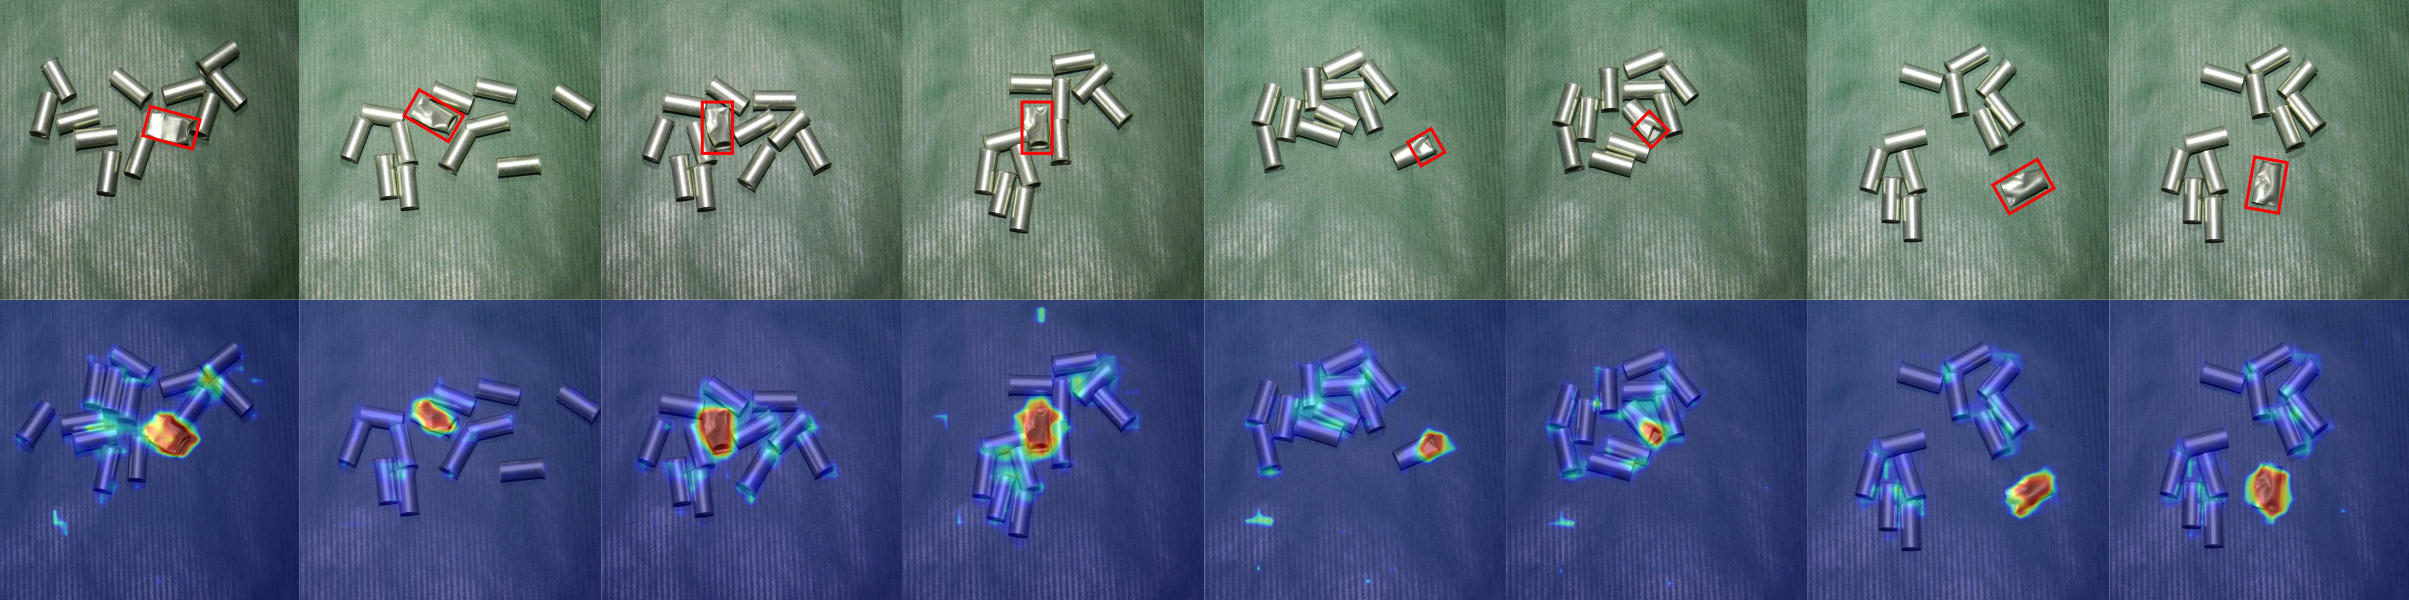
\includegraphics[width=\textwidth]{imgs/tubes.jpg}
  \caption{This visualization showcases the tube product from the MPDD dataset. The first row represents the input with the anomaly highlighted. The second row presents the segmentation results
from our model.}
   \label{fig:tubes}
\end{figure*}

\begin{figure*}
  \centering
  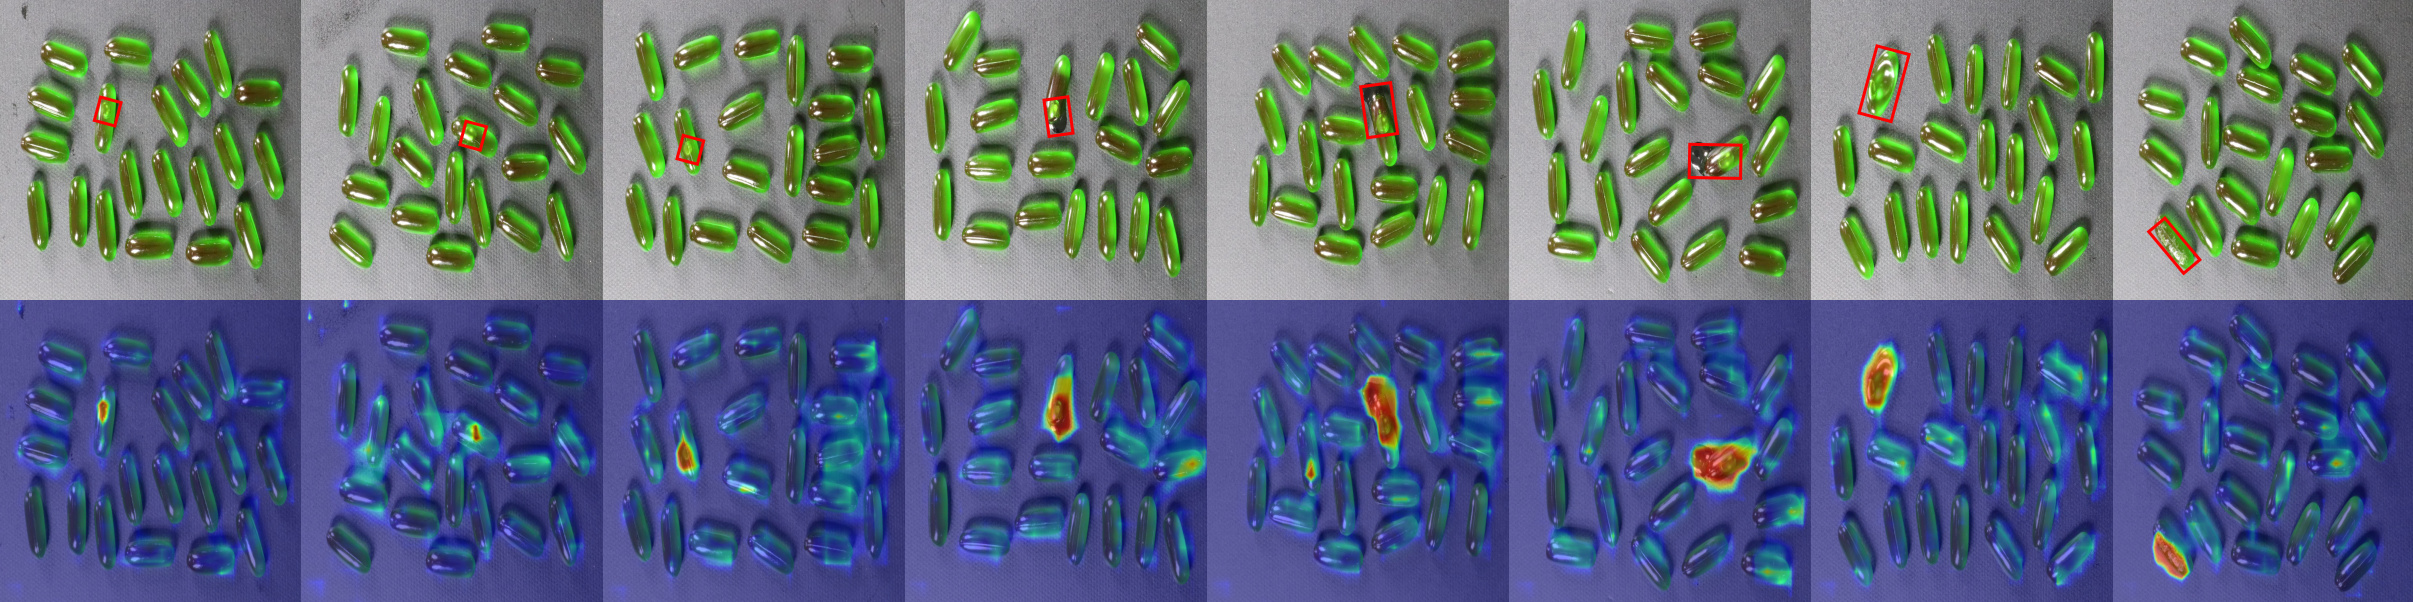
\includegraphics[width=\textwidth]{imgs/capsules.jpg}
  \caption{This visualization showcases the capsule product from the VisA dataset. The first row represents the input with the anomaly highlighted. The second row presents the segmentation results
from our model.}
   \label{fig:capsules}
\end{figure*}

\begin{figure*}
  \centering
  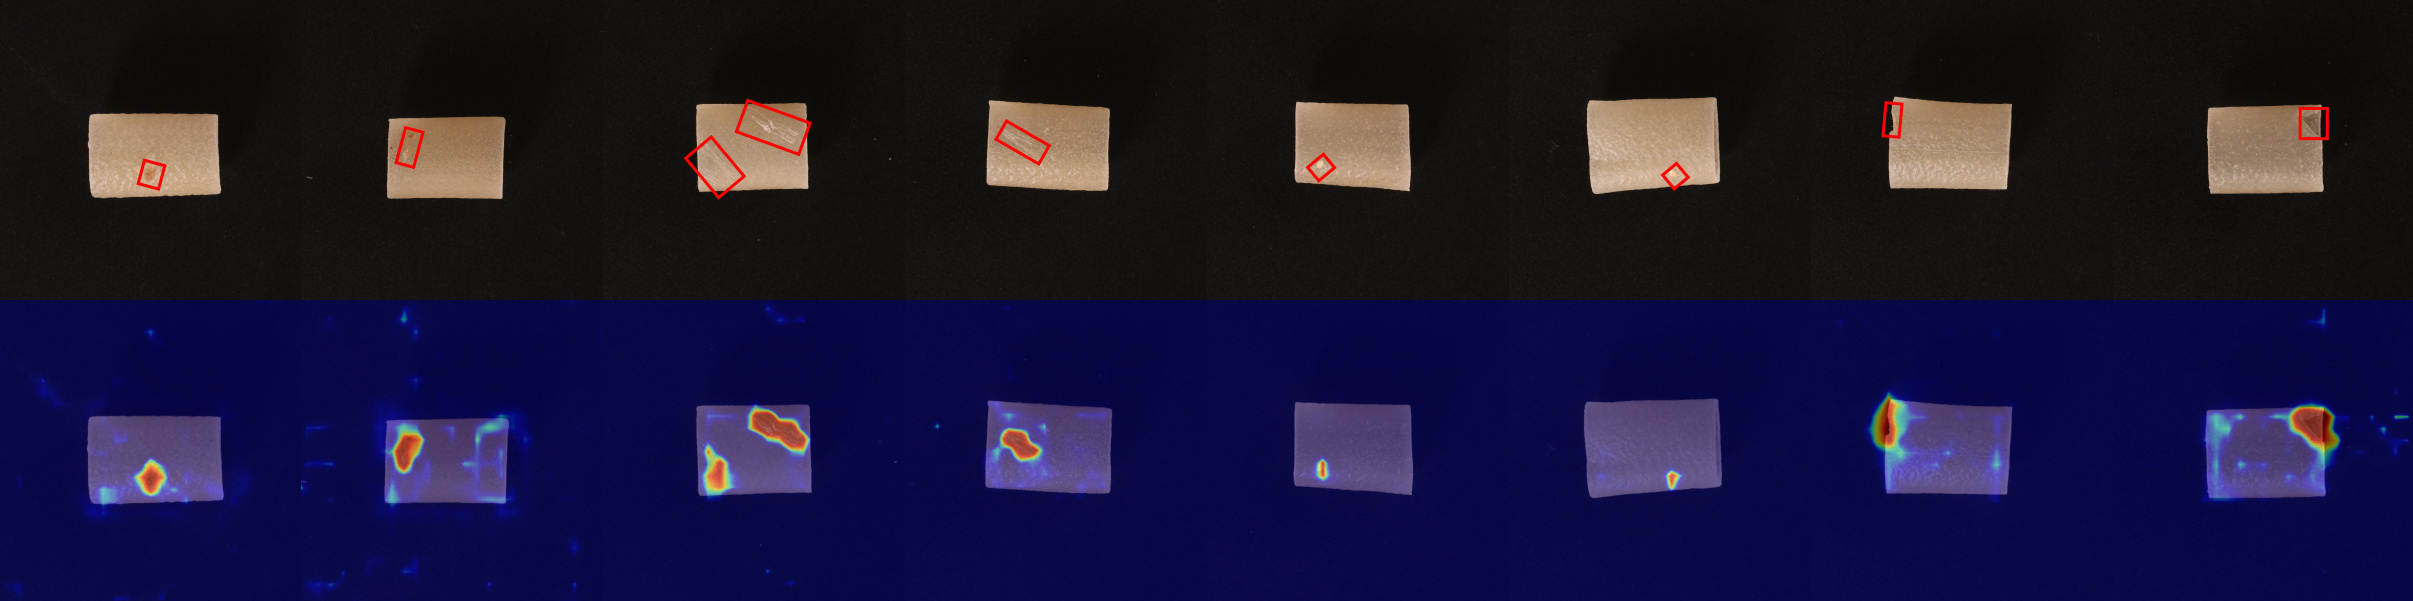
\includegraphics[width=\textwidth]{imgs/pipe-fryum.jpg}
  \caption{This visualization showcases the pipe fryum product from the VisA dataset. The first row represents the input with the anomaly highlighted. The second row presents the segmentation results
from our model.}
   \label{fig:pipe-fryum}
\end{figure*}

\begin{figure*}
  \centering
  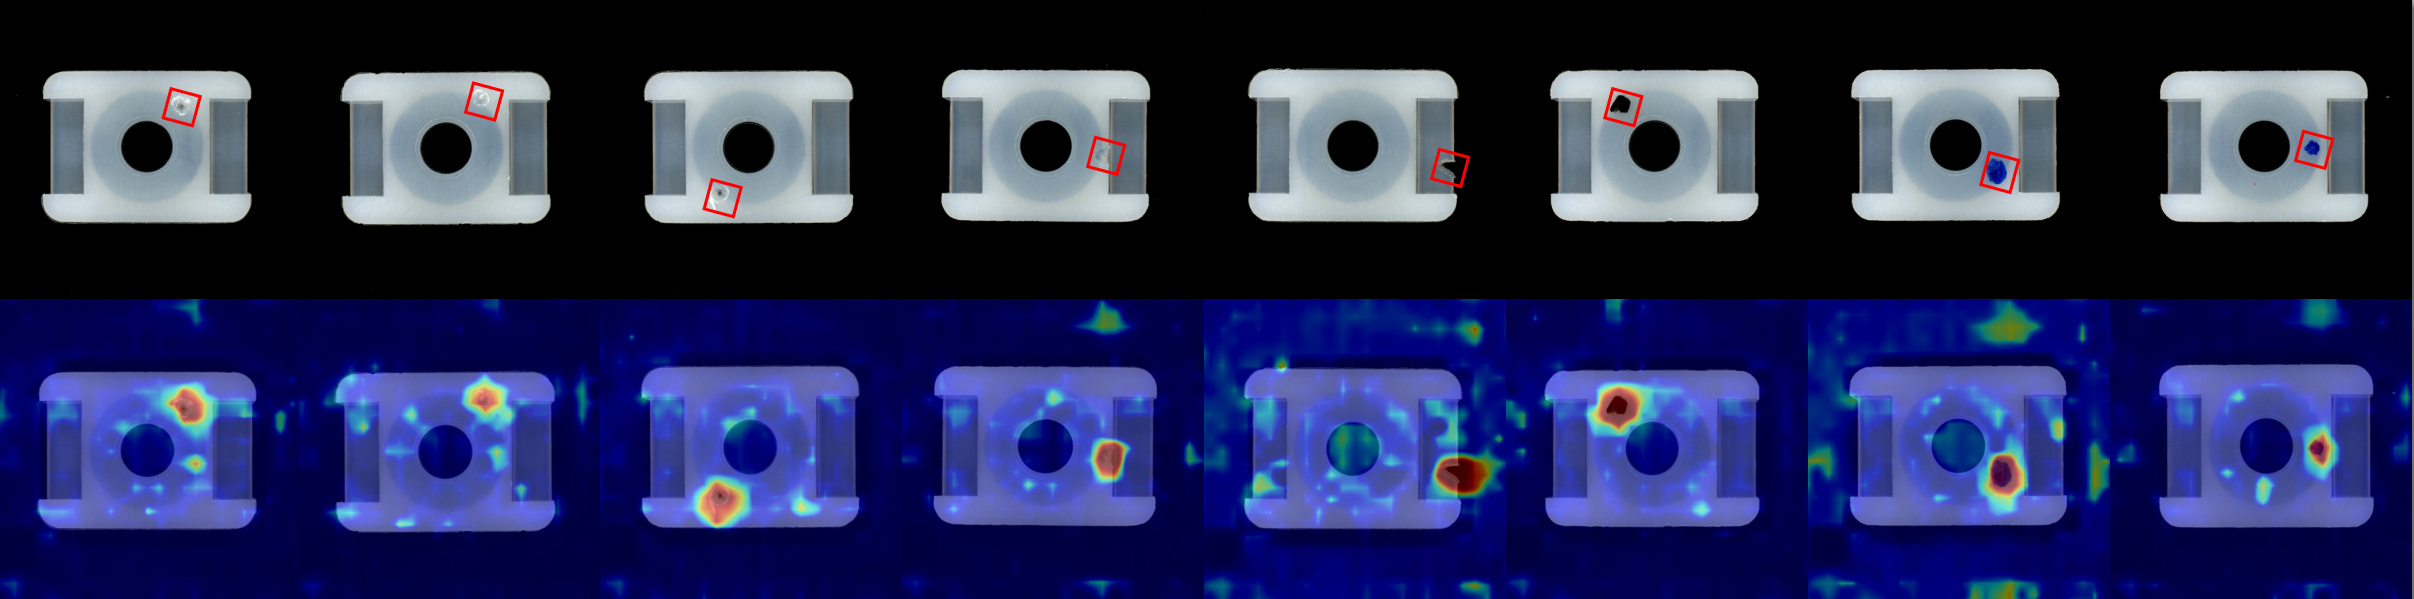
\includegraphics[width=\textwidth]{imgs/mounts.jpg}
  \caption{This visualization showcases the mount product from the Real-IAD dataset. The first row represents the input with the anomaly highlighted. The second row presents the segmentation results
from our model.}
   \label{fig:mounts}
\end{figure*}

\begin{figure*}
  \centering
  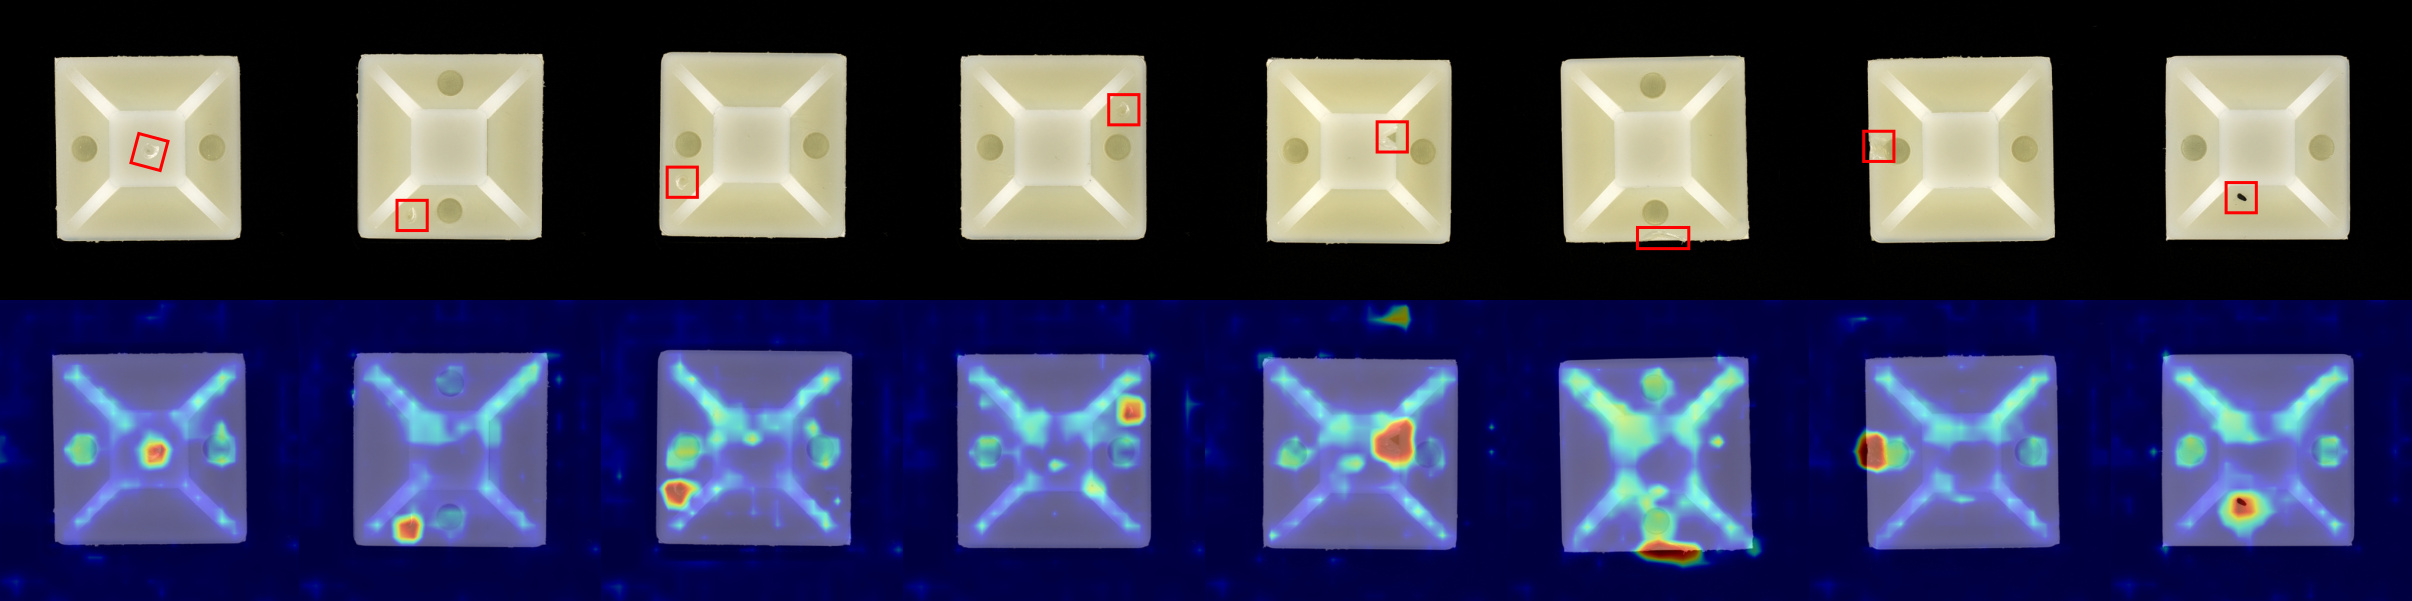
\includegraphics[width=\textwidth]{imgs/rolled_strip_base.jpg}
  \caption{This visualization showcases the rolled strip base product from the Real-IAD dataset. The first row represents the input with the anomaly highlighted. The second row presents the segmentation results
from our model.}
   \label{fig:rolled_strip_base}
\end{figure*}

\begin{figure*}
  \centering
  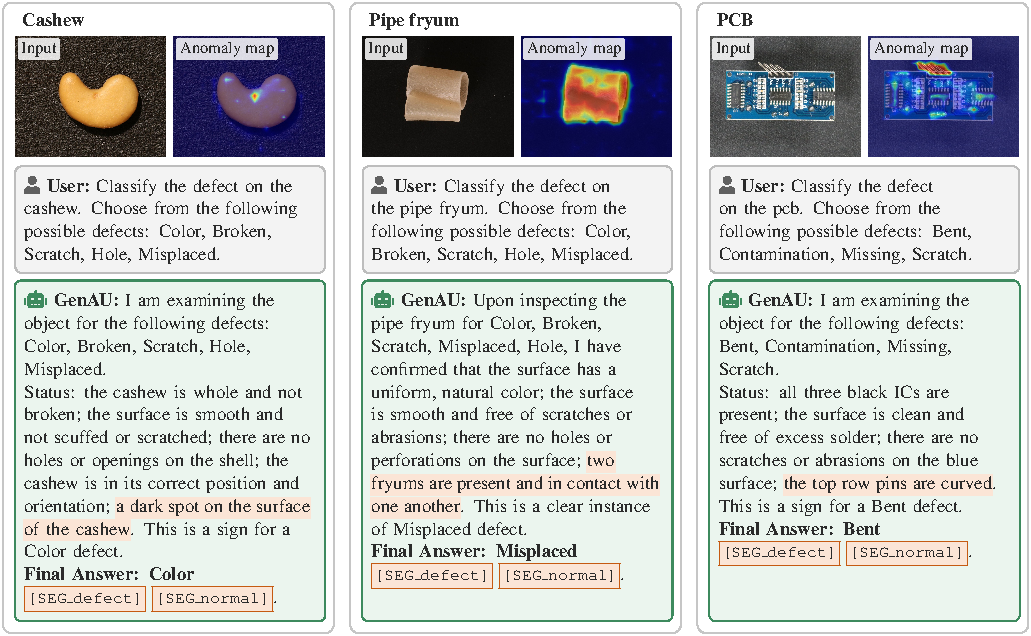
\includegraphics[width=\textwidth]{imgs/GenAU_Dialogue.pdf}
  \caption{This visualization showcases the abilities of GenAU. Given the input prompt and the image, the model reasons over the possible defects, identifies the correct one and outputs a segmentation mask.}
   \label{fig:text}
\end{figure*}

